\section{Experiments}
\label{sec:experiments}

\paragraph{Metrics.}
LoadCV is the coefficient of variation of expert usage; lower is closer to
uniform dispatch.  Max error is the largest absolute deviation from target
usage $1/E$.  NMI is normalized mutual information between evaluation-only
latent feature labels and routes; it is never used to build the router.  Margin
p05 is the fifth percentile of route margins.

\paragraph{Full-run setup.}
All results are full runs with five seeds.  E1 sweeps
$d\in\{32,64\}$, $E\in\{4,8\}$, and
$n_{\mathrm{cal}}\in\{2048,8192,16384\}$ with 8192 holdout points.  E2 uses
$d=64$, $E\in\{4,8\}$, and 8192 calibration/holdout points.  E3--E5 use
controlled feature populations with $E=8$ experts; E5 trains hard-routed
linear experts for 80 epochs.  Balanced assignment is always a forced-count
control, not a valid feature-only router.

\subsection{Static uniform dispatch}

E1 tests Gaussian and spherical features.  Table
\ref{tab:e1_static_dispatch} shows that SPR gives exact calibration balance and
low held-out imbalance.  Across the full sweep, the best SPR mean held-out
LoadCV is 0.034, compared with 0.086 for vanilla random linear routing.  Simplex
prototypes are strong on spherical data, which is expected because their
geometry matches the distribution.

\begin{table}[t]
\centering
\caption{Static uniform dispatch on the main full-run setting ($d=64$, $E=8$, largest calibration size).}
\label{tab:e1_static_dispatch}
\begin{tabular}{llrrrr}
\toprule
Data & Method & Cal LoadCV $\downarrow$ & Holdout LoadCV $\downarrow$ & Max error $\downarrow$ & Margin p05 $\uparrow$ \\
\midrule
Gaussian & Balanced assignment & 0.000 & 0.000 & 0.000 & -- \\
Gaussian & SPR-Expert & 0.000 & 0.036 & 0.009 & 0.022 \\
Gaussian & SPR-Fixed & 0.000 & 0.039 & 0.008 & 0.021 \\
Gaussian & SPR-Local & 0.000 & 0.041 & 0.009 & 0.021 \\
Gaussian & Simplex prototype & 0.015 & 0.031 & 0.006 & 0.038 \\
Gaussian & Vanilla linear & 0.068 & 0.072 & 0.015 & 0.035 \\
Spherical & Balanced assignment & 0.000 & 0.000 & 0.000 & -- \\
Spherical & SPR-Expert & 0.000 & 0.024 & 0.005 & 0.021 \\
Spherical & SPR-Fixed & 0.000 & 0.034 & 0.008 & 0.021 \\
Spherical & SPR-Local & 0.000 & 0.027 & 0.007 & 0.024 \\
Spherical & Simplex prototype & 0.020 & 0.029 & 0.007 & 0.039 \\
Spherical & Vanilla linear & 0.068 & 0.069 & 0.015 & 0.035 \\
\bottomrule
\end{tabular}
\end{table}


\begin{figure}[t]
\centering
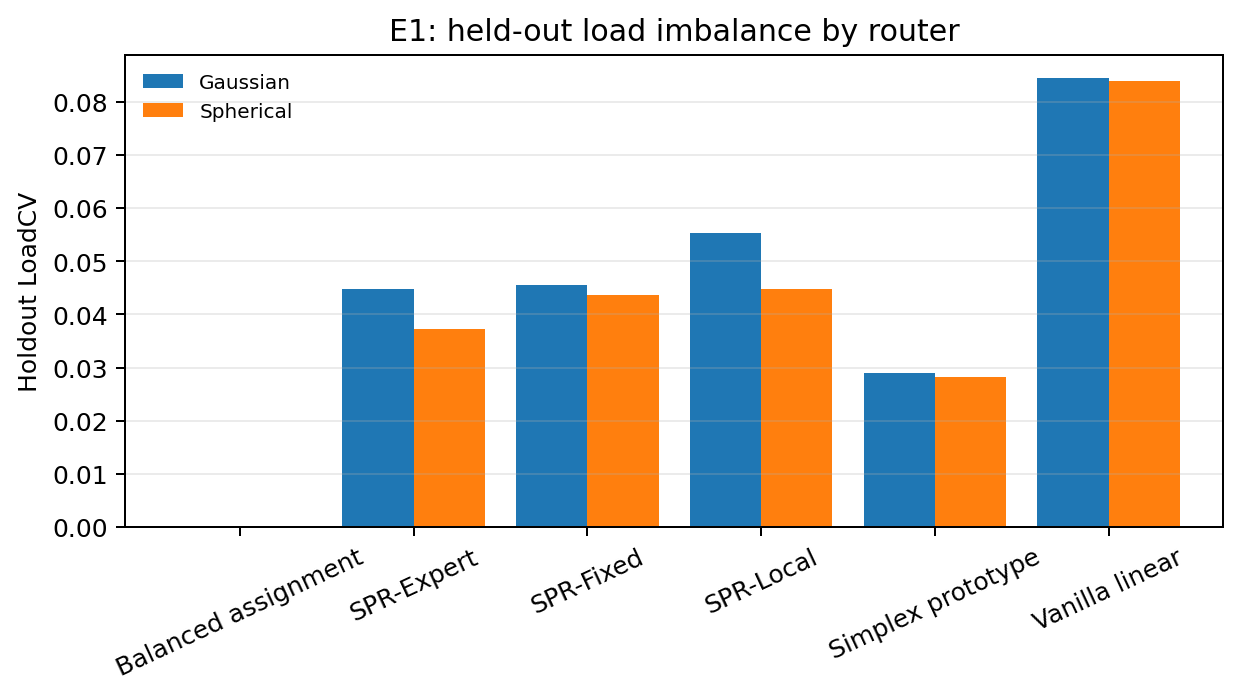
\includegraphics[width=0.48\linewidth]{figures/e1_loadcv_by_method.png}
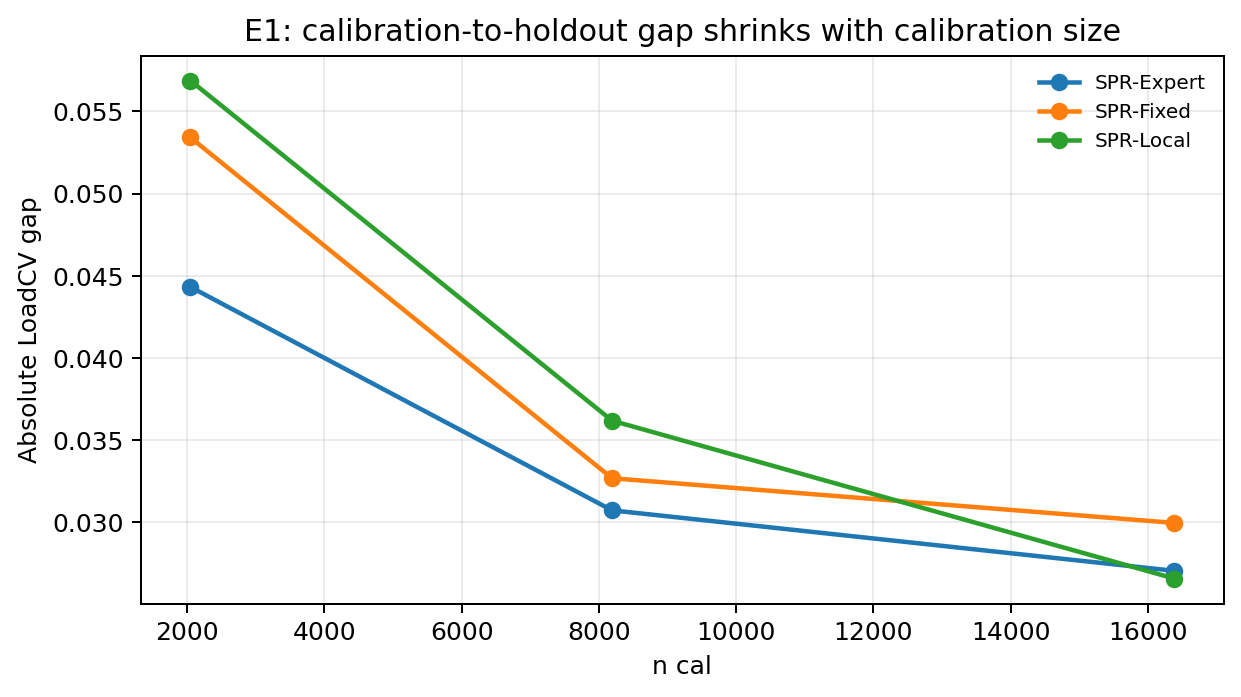
\includegraphics[width=0.48\linewidth]{figures/e1_holdout_gap.png}
\caption{E1 static dispatch. Left: held-out usage imbalance. Right:
calibration-to-holdout gap for SPR variants.}
\label{fig:e1_static}
\end{figure}

\subsection{Covariance-flat non-spherical features}

E2 tests whitened axis-jitter, sparse-mixture, and paired-direction features.
Their covariance condition number is 1.00, yet prototype-router cells can have
unequal probability mass.  On axis-supported features, simplex prototype
routing reaches LoadCV 0.752, while SPR variants are near 0.04.  The paired
direction case is a boundary case because finite support and near-ties make
deterministic feature-only splitting unstable.

\begin{table}[t]
\centering
\caption{Spectrally flat but non-spherical features. Covariance flatness alone does not force prototype-router balance.}
\label{tab:e2_non_spherical}
\begin{tabular}{lrrlrr}
\toprule
Data & Cond. $\downarrow$ & Eff. rank $\uparrow$ & Method & LoadCV $\downarrow$ & Max error $\downarrow$ \\
\midrule
Axis-jitter & 1.00 & 64.0 & Balanced assignment & 0.000 & 0.000 \\
Axis-jitter & 1.00 & 64.0 & SPR-Expert & 0.039 & 0.009 \\
Axis-jitter & 1.00 & 64.0 & SPR-Fixed & 0.044 & 0.010 \\
Axis-jitter & 1.00 & 64.0 & SPR-Local & 0.039 & 0.008 \\
Axis-jitter & 1.00 & 64.0 & Simplex prototype & 0.752 & 0.215 \\
Axis-jitter & 1.00 & 64.0 & Vanilla linear & 0.162 & 0.034 \\
Paired-directions & 1.00 & 64.0 & Balanced assignment & 0.000 & 0.000 \\
Paired-directions & 1.00 & 64.0 & SPR-Expert & 0.180 & 0.038 \\
Paired-directions & 1.00 & 64.0 & SPR-Fixed & 0.211 & 0.047 \\
Paired-directions & 1.00 & 64.0 & SPR-Local & 0.199 & 0.046 \\
Paired-directions & 1.00 & 64.0 & Simplex prototype & 0.136 & 0.028 \\
Paired-directions & 1.00 & 64.0 & Vanilla linear & 0.173 & 0.043 \\
Sparse-mixture & 1.00 & 64.0 & Balanced assignment & 0.000 & 0.000 \\
Sparse-mixture & 1.00 & 64.0 & SPR-Expert & 0.031 & 0.007 \\
Sparse-mixture & 1.00 & 64.0 & SPR-Fixed & 0.031 & 0.008 \\
Sparse-mixture & 1.00 & 64.0 & SPR-Local & 0.049 & 0.010 \\
Sparse-mixture & 1.00 & 64.0 & Simplex prototype & 0.188 & 0.044 \\
Sparse-mixture & 1.00 & 64.0 & Vanilla linear & 0.088 & 0.021 \\
\bottomrule
\end{tabular}
\end{table}


\begin{figure}[t]
\centering
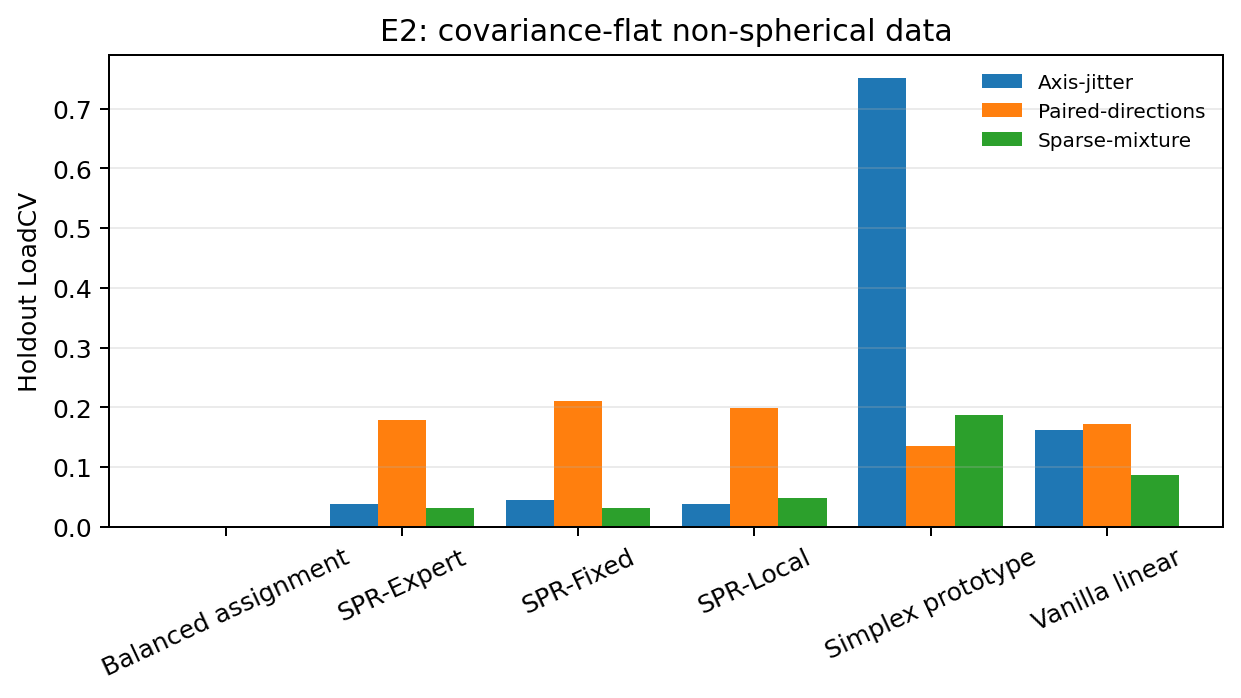
\includegraphics[width=0.48\linewidth]{figures/e2_non_spherical_loadcv.png}
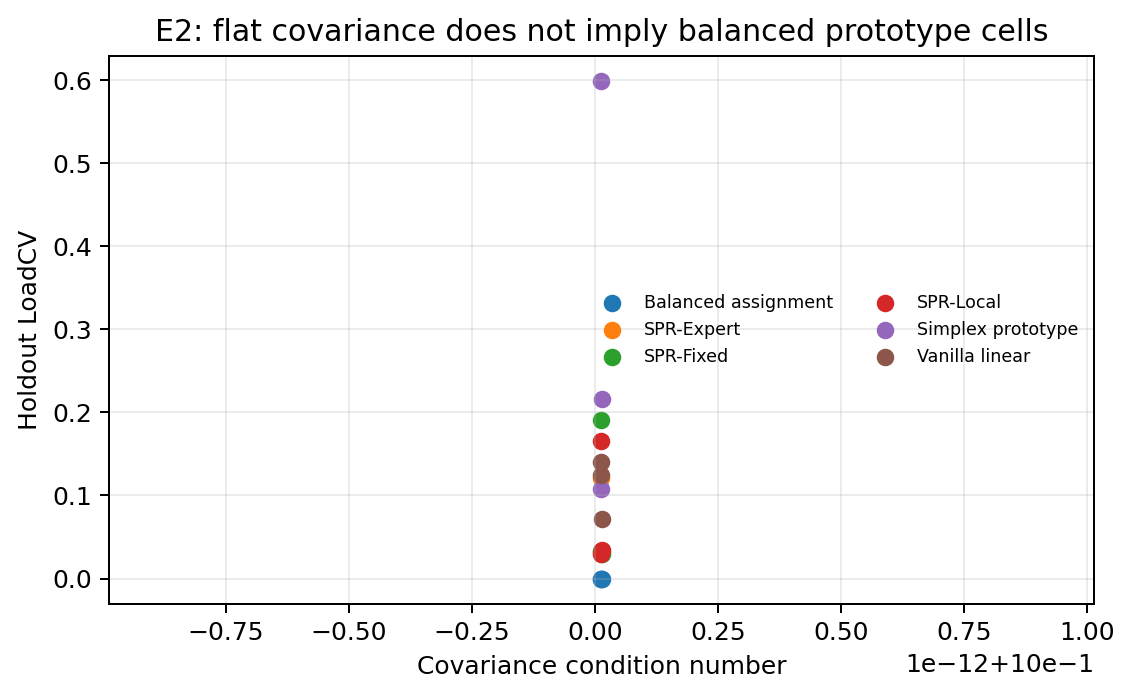
\includegraphics[width=0.48\linewidth]{figures/e2_covariance_vs_load.png}
\caption{E2 non-spherical features. Flat covariance does not determine the
probability mass of prototype-router cells.}
\label{fig:e2_non_spherical}
\end{figure}

\subsection{Expert-weight guidance}

E3 tests random, symmetric, and clustered expert matrices.  We extract expert
principal directions by SVD or one-step power iteration.  Prototype-only top-1
routing aligns with expert directions but does not control mass.  SPR-Expert
uses the same prototypes only to choose split directions; quantiles choose
thresholds.  Table \ref{tab:e3_expert_guided} shows that SPR-Expert reaches
mean held-out LoadCV 0.018 and cell-to-prototype alignment 0.895, while
expert-SVD top-1 has alignment 0.910 but LoadCV 0.111.

\begin{table}[t]
\centering
\caption{Expert-weight-guided routing. Expert prototypes improve alignment, while quantile thresholds control mass.}
\label{tab:e3_expert_guided}
\begin{tabular}{llrrrr}
\toprule
Expert init & Router & Proto spread $\uparrow$ & Alignment $\uparrow$ & LoadCV $\downarrow$ & Margin p05 $\uparrow$ \\
\midrule
clustered & Expert-SVD top-1 & 0.877 & 0.903 & 0.149 & 0.039 \\
clustered & MPI one-step top-1 & 0.877 & 0.909 & 0.094 & 0.035 \\
clustered & SPR-Expert & 0.877 & 0.884 & 0.021 & 0.022 \\
clustered & SPR-Expert-MPI & 0.877 & 0.896 & 0.021 & 0.022 \\
clustered & SPR-Local & 0.877 & 0.098 & 0.021 & 0.021 \\
random & Expert-SVD top-1 & 0.894 & 0.934 & 0.070 & 0.035 \\
random & MPI one-step top-1 & 0.894 & 0.931 & 0.075 & 0.035 \\
random & SPR-Expert & 0.894 & 0.917 & 0.017 & 0.021 \\
random & SPR-Expert-MPI & 0.894 & 0.911 & 0.015 & 0.021 \\
random & SPR-Local & 0.894 & 0.087 & 0.024 & 0.022 \\
symmetric & Expert-SVD top-1 & 0.875 & 0.893 & 0.113 & 0.038 \\
symmetric & MPI one-step top-1 & 0.875 & 0.915 & 0.084 & 0.036 \\
symmetric & SPR-Expert & 0.875 & 0.886 & 0.016 & 0.024 \\
symmetric & SPR-Expert-MPI & 0.875 & 0.898 & 0.021 & 0.021 \\
symmetric & SPR-Local & 0.875 & 0.098 & 0.019 & 0.021 \\
\bottomrule
\end{tabular}
\end{table}


\begin{figure}[t]
\centering
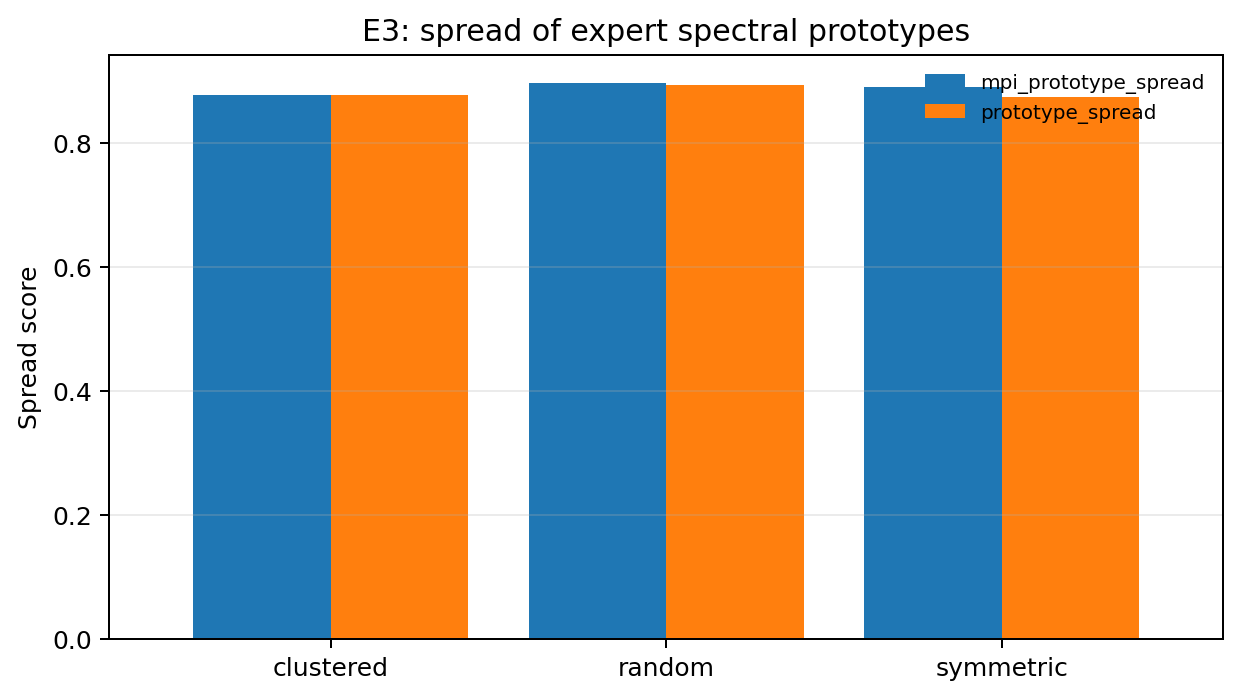
\includegraphics[width=0.48\linewidth]{figures/e3_prototype_spread.png}
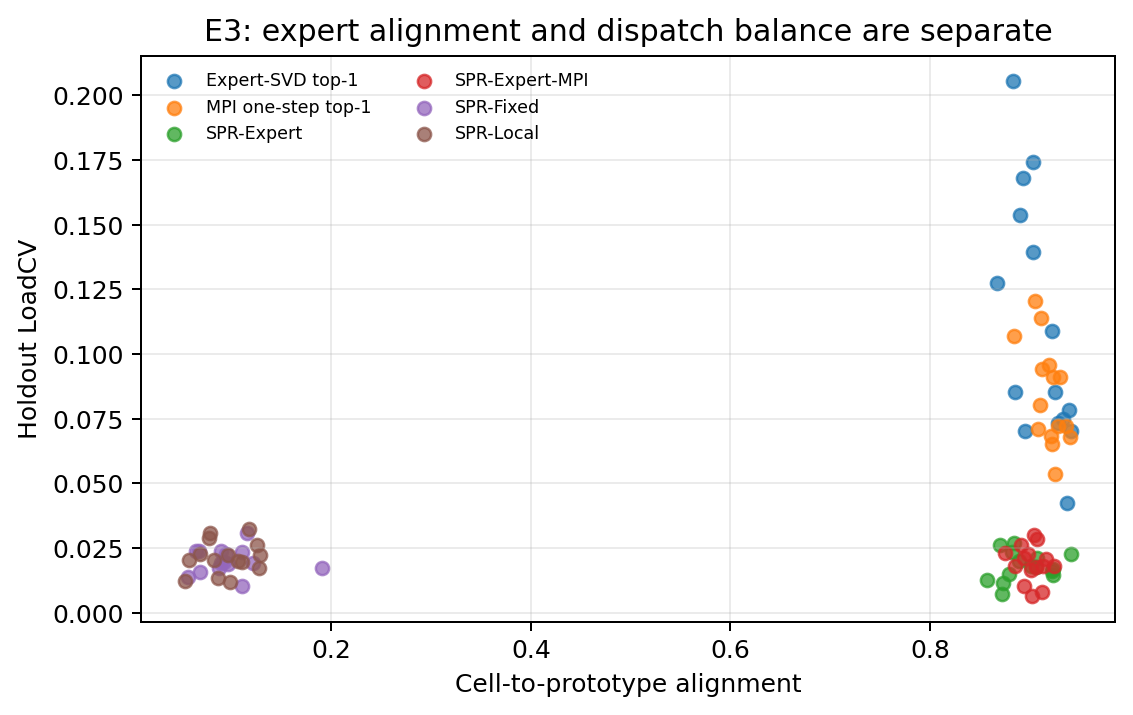
\includegraphics[width=0.48\linewidth]{figures/e3_alignment_vs_loadcv.png}
\caption{E3 expert guidance. Expert prototypes provide geometry, but quantile
thresholds are needed for low usage imbalance.}
\label{fig:e3_expert}
\end{figure}

\subsection{Feature partition quality}

E4 separates count balance from meaningful feature partition.  We generate
balanced latent feature classes, randomly rotate the geometry, whiten globally,
and hide labels from all routers.  Table \ref{tab:e4_feature_partition} shows
that balanced assignment has perfect counts but NMI 0.007.  SPR-Fixed and
SPR-Local are also near random in NMI.  SPR-Expert improves NMI to 0.233 and
purity to 0.408 because its expert weights contain directions aligned with the
latent geometry.  This supports expert-guided geometry, not a broad claim that
locality-only quantile cuts recover the right classes.

\begin{table}[t]
\centering
\caption{Feature partition quality on evaluation-only latent classes.}
\label{tab:e4_feature_partition}
\begin{tabular}{lrrrrr}
\toprule
Method & LoadCV $\downarrow$ & NMI $\uparrow$ & Purity $\uparrow$ & Within-var. $\downarrow$ & Margin p05 $\uparrow$ \\
\midrule
Balanced assignment & 0.000 & 0.007 & 0.153 & 63.137 & -- \\
SPR-Expert & 0.015 & 0.233 & 0.408 & 62.014 & 0.021 \\
SPR-Fixed & 0.019 & 0.031 & 0.199 & 62.172 & 0.021 \\
SPR-Local & 0.021 & 0.034 & 0.219 & 62.152 & 0.022 \\
Simplex prototype & 0.017 & 0.029 & 0.198 & 61.764 & 0.038 \\
Vanilla linear & 0.089 & 0.033 & 0.196 & 61.774 & 0.036 \\
\bottomrule
\end{tabular}
\end{table}


\begin{figure}[t]
\centering
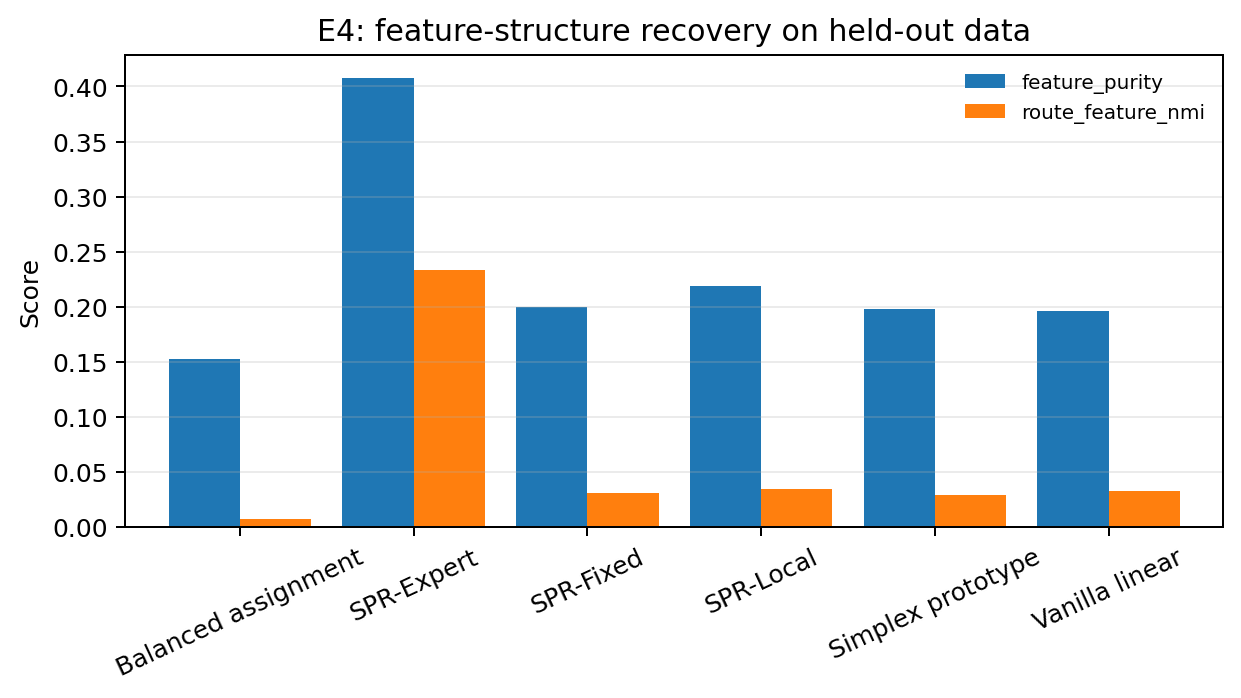
\includegraphics[width=0.48\linewidth]{figures/e4_nmi_purity.png}
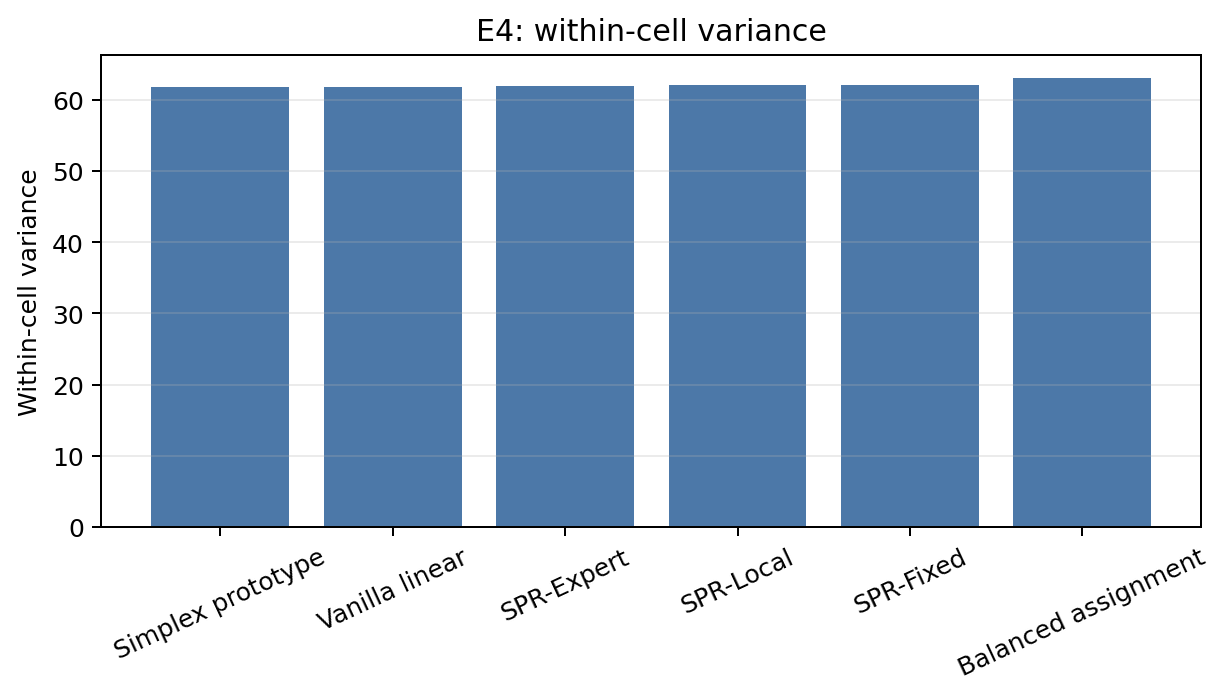
\includegraphics[width=0.48\linewidth]{figures/e4_within_cell_variance.png}
\caption{E4 feature partition quality. Count balance is not enough; alignment
requires a geometry source that matches latent feature structure.}
\label{fig:e4_quality}
\end{figure}

\subsection{Controlled training dynamics}

E5 uses a hard-routing regression task where each latent feature class has a
different target map, $Y=A_FX+\epsilon$.  The routers never observe $F$.
Experts train under the routes produced by each method.  SPR-Expert reaches
final validation MSE 9.03 and NMI 0.385; vanilla linear routing reaches MSE
12.61 and NMI 0.087.  SlowUpdate-SPR is a negative result: repeated
recalibration gives route flip rate 0.888 and worse loss.

\begin{table}[t]
\centering
\caption{Controlled hard-routing expert training at the final epoch.}
\label{tab:e5_training_dynamics}
\begin{tabular}{lrrrrrr}
\toprule
Router & Val MSE $\downarrow$ & LoadCV $\downarrow$ & NMI $\uparrow$ & Flip $\downarrow$ & Margin p05 $\uparrow$ & Spec. $\uparrow$ \\
\midrule
Frozen-SPR & 12.472 & 0.050 & 0.077 & 0.025 & 0.021 & 0.268 \\
Linear + load-balance & 13.292 & 0.000 & 0.038 & 0.049 & -- & 0.197 \\
SPR-Expert & 9.030 & 0.047 & 0.385 & 0.024 & 0.024 & 0.514 \\
SPR-init-linear & 11.558 & 0.053 & 0.179 & 0.020 & 0.041 & 0.392 \\
Simplex init & 12.442 & 0.044 & 0.089 & 0.022 & 0.039 & 0.266 \\
SlowUpdate-SPR & 17.432 & 0.053 & 0.096 & 0.888 & 0.022 & 0.301 \\
Vanilla linear & 12.613 & 0.107 & 0.087 & 0.023 & 0.035 & 0.267 \\
\bottomrule
\end{tabular}
\end{table}


\begin{figure}[t]
\centering
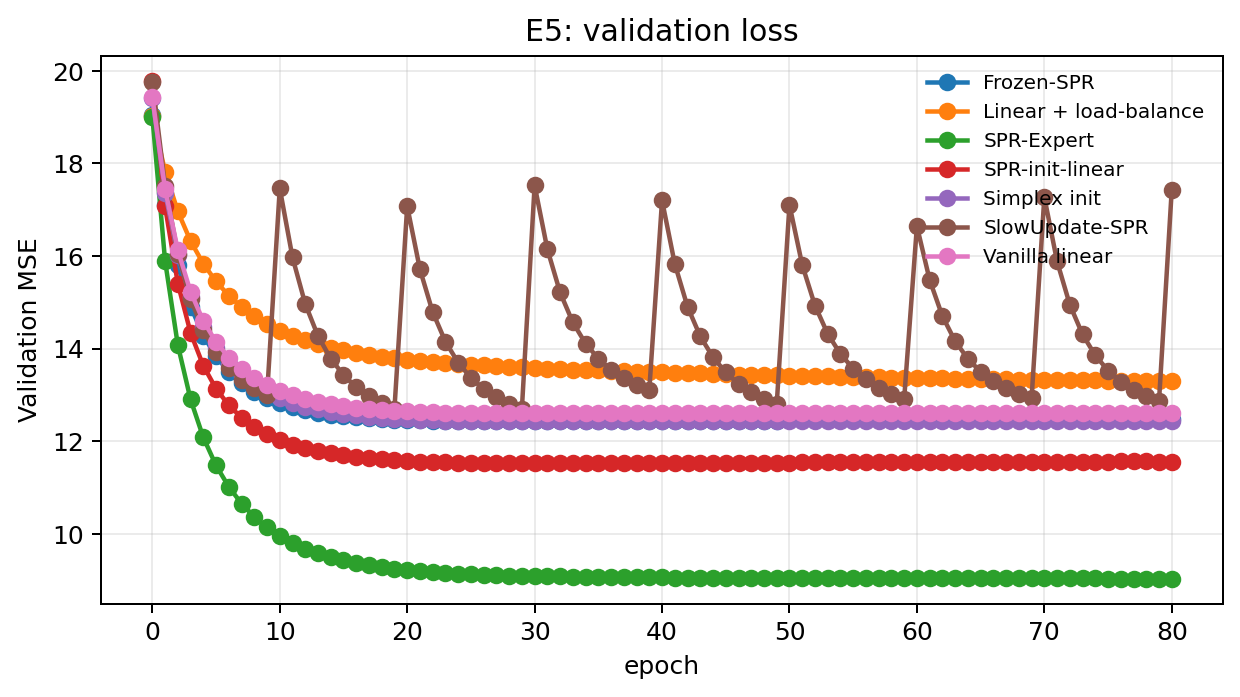
\includegraphics[width=0.48\linewidth]{figures/e5_loss_curves.png}
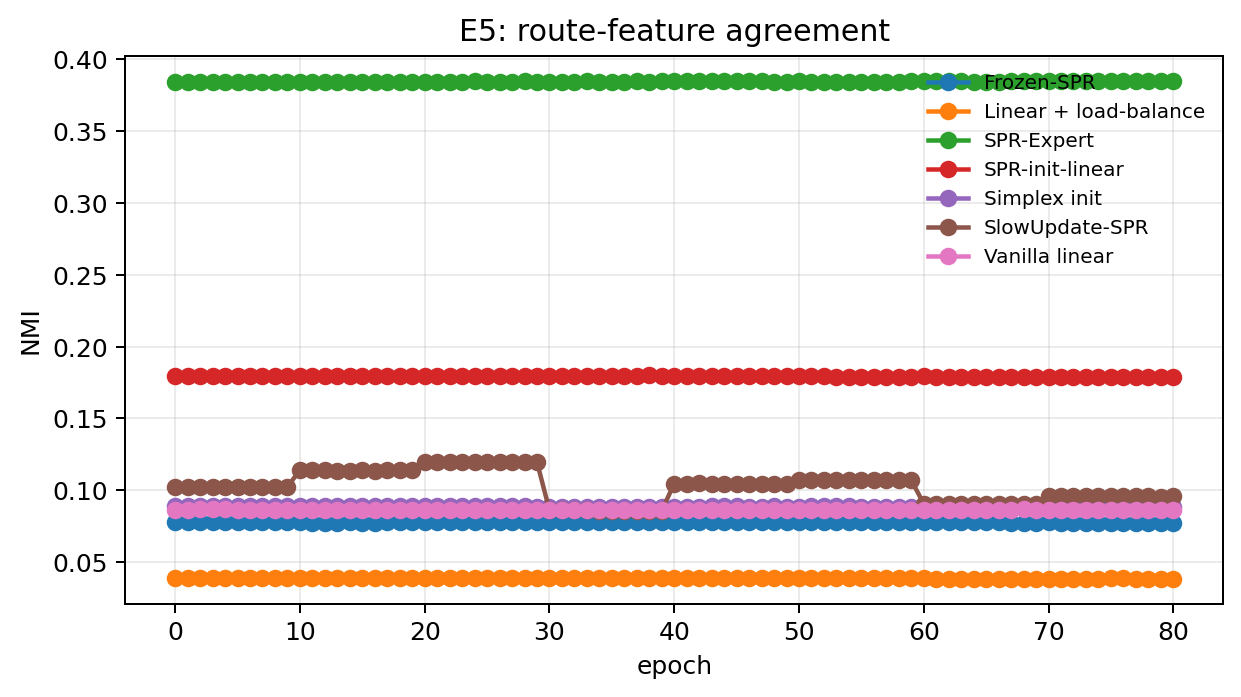
\includegraphics[width=0.48\linewidth]{figures/e5_route_nmi.png}
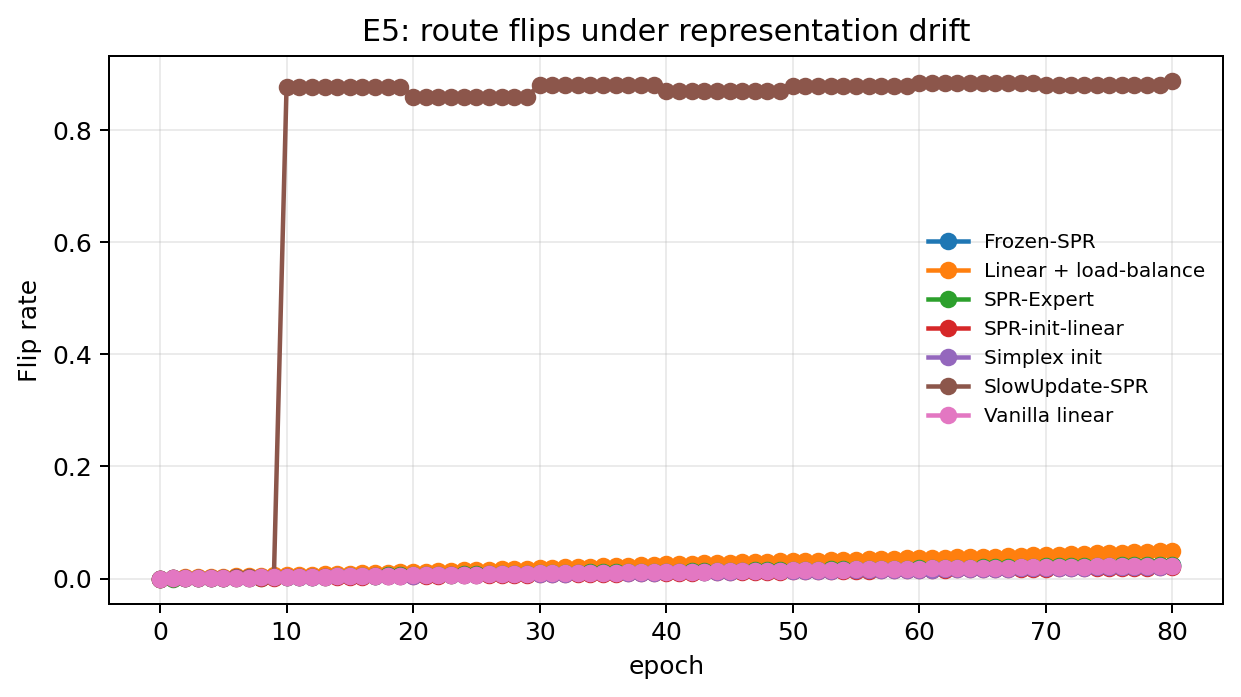
\includegraphics[width=0.48\linewidth]{figures/e5_flip_rate.png}
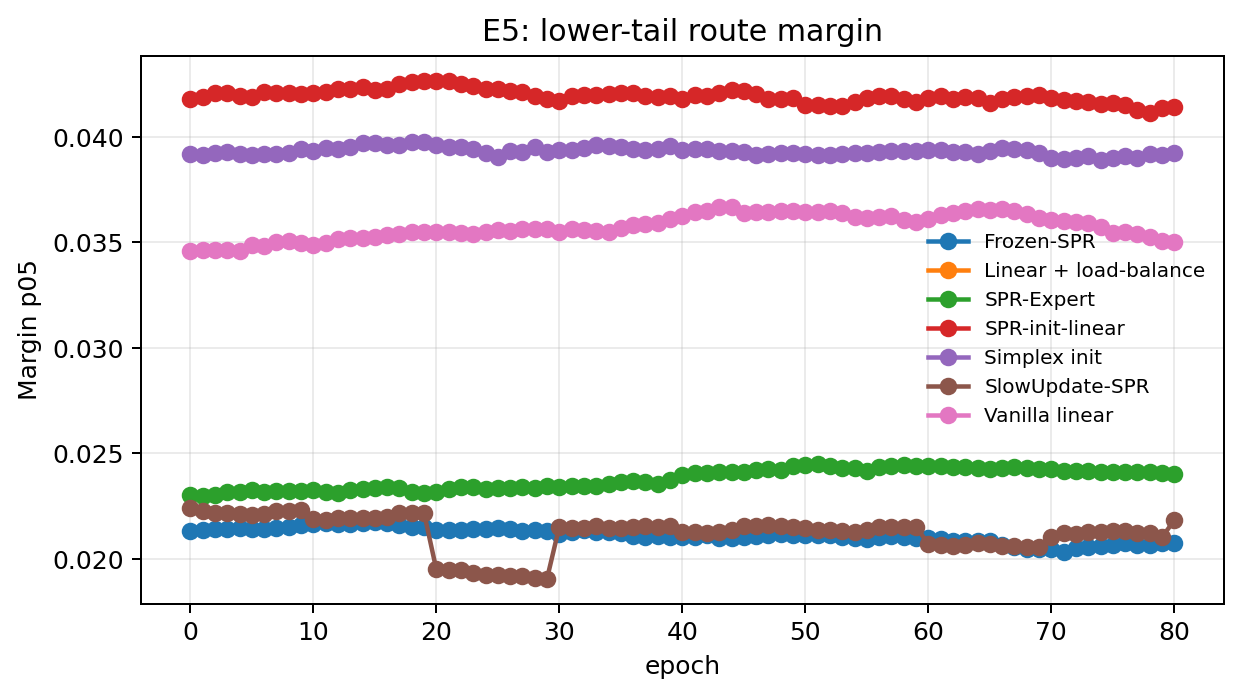
\includegraphics[width=0.48\linewidth]{figures/e5_margin_p05.png}
\caption{E5 controlled training dynamics. Expert-guided geometry improves the
controlled task, while naive slow recalibration creates route instability.}
\label{fig:e5_training}
\end{figure}

\subsection{Ablations}

E6 audits calibration size, dimension, expert count, direction policy,
whitening, expert quality, count forcing, and drift.  Larger calibration sets
improve held-out balance: LoadCV drops from 0.089 at
$n_{\mathrm{cal}}=512$ to 0.025 at 32768.  Expert quality controls feature
agreement: aligned expert weights give NMI 0.282, while noisy or random weights
collapse near fixed/local baselines.

\begin{table}[t]
\centering
\caption{Ablations and boundary checks.}
\label{tab:e6_ablations}
\begin{tabular}{llrrrr}
\toprule
Ablation & Setting & LoadCV $\downarrow$ & NMI $\uparrow$ & Margin p05 $\uparrow$ & Max error $\downarrow$ \\
\midrule
calibration\_size & 2048 & 0.077 & 0.025 & 0.021 & 0.020 \\
calibration\_size & 32768 & 0.025 & 0.032 & 0.021 & 0.006 \\
calibration\_size & 512 & 0.089 & 0.035 & 0.023 & 0.019 \\
calibration\_size & 8192 & 0.025 & 0.026 & 0.021 & 0.005 \\
count\_control & feature\_router & 0.029 & 0.031 & 0.021 & 0.006 \\
count\_control & forced\_count & 0.000 & 0.012 & -- & 0.000 \\
dimension & 128 & 0.025 & 0.015 & 0.021 & 0.006 \\
dimension & 16 & 0.034 & 0.172 & 0.023 & 0.007 \\
dimension & 32 & 0.028 & 0.076 & 0.022 & 0.007 \\
dimension & 64 & 0.029 & 0.032 & 0.021 & 0.007 \\
direction\_policy & expert & 0.028 & 0.255 & 0.022 & 0.007 \\
direction\_policy & fixed & 0.027 & 0.033 & 0.021 & 0.006 \\
direction\_policy & local & 0.038 & 0.037 & 0.021 & 0.009 \\
expert\_count & 12 & 0.040 & 0.034 & 0.017 & 0.007 \\
expert\_count & 4 & 0.022 & 0.013 & 0.032 & 0.009 \\
expert\_count & 6 & 0.028 & 0.020 & 0.025 & 0.008 \\
expert\_count & 8 & 0.030 & 0.029 & 0.021 & 0.006 \\
expert\_weight\_quality & aligned & 0.035 & 0.232 & 0.022 & 0.008 \\
expert\_weight\_quality & noisy & 0.034 & 0.027 & 0.021 & 0.008 \\
expert\_weight\_quality & random & 0.040 & 0.021 & 0.021 & 0.009 \\
feature\_drift & 0.00 & 0.037 & 0.029 & 0.021 & 0.009 \\
feature\_drift & 0.05 & 0.038 & 0.029 & 0.021 & 0.009 \\
feature\_drift & 0.15 & 0.037 & 0.029 & 0.022 & 0.009 \\
feature\_drift & 0.30 & 0.036 & 0.029 & 0.022 & 0.009 \\
whitening & off & 0.030 & 0.094 & 0.025 & 0.007 \\
whitening & on & 0.034 & 0.031 & 0.020 & 0.008 \\
\bottomrule
\end{tabular}
\end{table}


\begin{figure}[t]
\centering
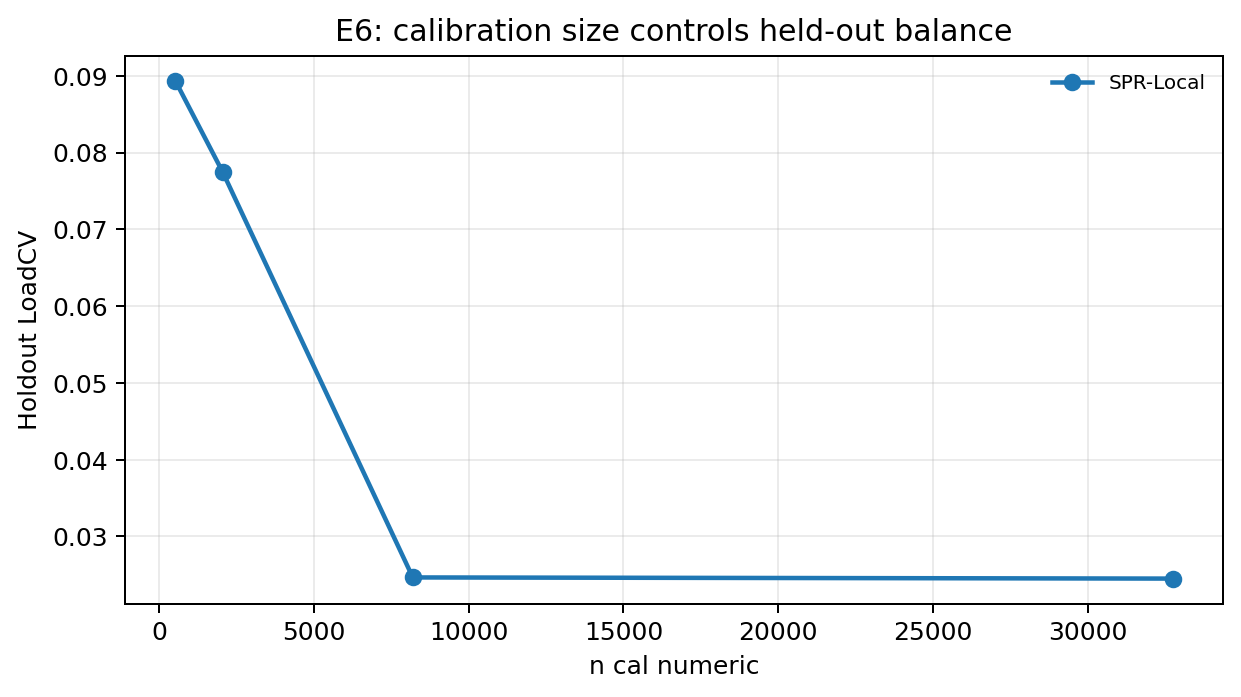
\includegraphics[width=0.48\linewidth]{figures/e6_calibration_size.png}
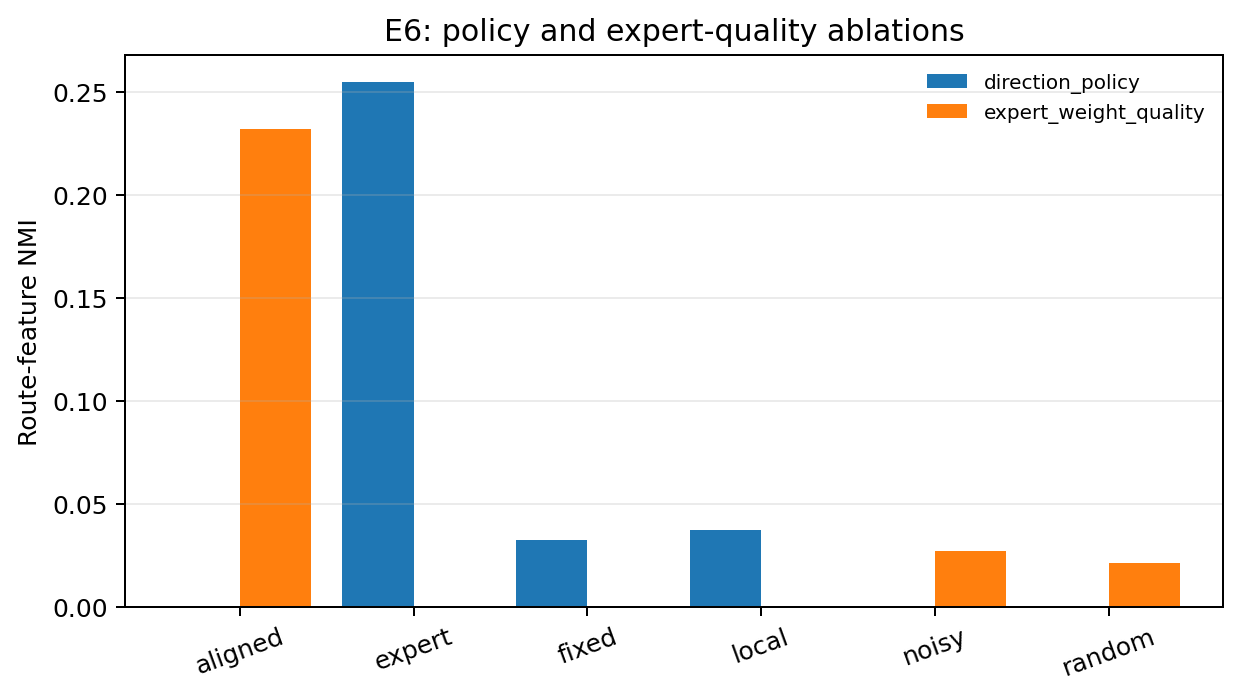
\includegraphics[width=0.48\linewidth]{figures/e6_policy_ablation.png}
\caption{E6 ablations. Calibration size controls statistical balance; expert
weight quality controls feature agreement.}
\label{fig:e6_ablations}
\end{figure}

\FloatBarrier
